\chapter{Simulation comparison \& evaluations}
In the previous chapter we have described our model, with the reactive concession strategy. Here the reactive concession strategy is compared to a non-reactive concession strategy. Furthermore different values for the reservation utility are checked, and different values for the mixbed agent water requirements are compared. 

\section{Parameters}
The parameters that are checked are compared to the baseline non-reactive strategy. Firstly the Nash solution is described to compare to the optimal solution. The parameters will be described in more detail.

\subsection{Nash Bargaining Solution}
The Nash bargaining solution is found using the product of agent's utility, maximizing the joint utility: $\prod_{i=i}^{m}u_i(x).$ We can calculate this since to us the utilities of the agent is known. This information is unknown to the agents since they only know their own utility curve. The joint utility gives the global maximum, and optimal Nash Solution. The utility functions of the agents are convex, which means that the solution is Pareto optimal and maximizes the product of the utilities \citep{nash1950bargaining, roth1977individual, lensberg1988stability}. 

\begin{alignat*}{2}
\text{maximize }   	& \prod_{i=1}^m u_i(x)  \\
\text{subject to \ } 	& u_i(x) \geq ru_i, & i = 1,...,m\\
& 0\leq x_j\leq 1, & j = 1,...,n\\
\end{alignat*}

Using the GAMS solver, the solutions are calculated. The limit for the reservation curve is also found, $\forall i,  ru_i = 0.3182$. This means that there is no solution space, if $\forall i, ru_i > 0.3182$. However, if only a single agent were to have a $ru_i > 0.3182$, there still would be a solution. This obviously depends on the reservation curve values of the other agents. \todo[show the nash solution visualised?]{Show the nash solution visualised?}

\subsection{Non-reactive concession strategy}
As explained in \Cref{sec:concessionstrat} the concession strategy determines whether a solution will be found. If no concession is made during the negotiation, and the agent stay on their initial utility, no agreement can be made. In this result the non-reactive strategy is used as a base line to compare to other methods. As described, there are a large number of different methods, and a weak concession is used in here, since the utility functions of the other agents are unknown. The non-reactive concession strategy used is $s_i(t) = \max \{s_0(t) - t * 0.01, ru_i\}$. This monotonic decreasing concession is a linear function until the reservation value. Described by \cite{wu2009efficient}, it is an \textit{amount of utility}, where Agent $ i \in N$ concedes a fixed amount utility $au$. Since the utility functions are private, utilitarian concessions are not possible \citep{endriss2006monotonic}. 

This means that the minimum utility value is reached after 100 rounds, if only the non-reactive concession strategy is used. Then each agent makes $\frac{100}{4 \text{agents}} = 25 \text{proposals}$. Since we combine it with the reactive concession strategy, it is possible for the agents to negotiate for more rounds.

\subsection{Reactive Concession strategy}
The reactive concession strategy (see \Cref{sec:reactiveconcessionstr} for an explanation) is compared to the non-reactive concession strategy. Similar to \citet{zheng2015automated}, however here different reservation utilities are checked, while comparing the reactive to non-reactive strategy.

\subsection{Reservation curve}
The curve, as shown in \Cref{sec:design:negmod}, is not really a curve, but a linear limit. The values can differ from 	
$ru_i = \{0.05, 0.10, 0.15, 0.20, 0.25, 0.3, 0.35, 0.4, 0.45, 0.5, \\0.55, 0.6, 0.65\}$. We have seen that in the initial case, there is no agreement zone if the $ru_i$ is larger than $0.3182$. But, since we try different kind of parameters, it could be the case that if one of the reservation curves were to be different, the rest could as well. 

\subsection{Distance}
For the algorithm \Cref{al:algorithm1} to finish, there are two option. Either the distance from the offer and weight is smaller than a threshold, or max number of rounds are reached. This distance, $\max_{ j \in {1,2,...,m}} \parallel x^j_t-w_{t-1} \parallel$ gives the maximum distance from the agents to the weight. It tells something about the final solution and is thus used in the results to determine how the efficiency of the solutions. 

If the distance is larger than the threshold, it means that the agents have not found an agreement and the max number of rounds has been reached. The final solution will be the average of all proposals. Two options are possible. Either one or more agent(s) has not conceded and thus not moved to the agreement-zone. Another option is that the reservation utilities is too high, meaning that there is no agreement-zone, and thus no agreement possible. 

Since we know where the agreement zone lies, we can see when the agent(s) do not concede, and thus refrain from agreement if the distance is larger than the threshold.


\subsubsection{Threshold \& maximum number of rounds}
As shown in the algorithm, there is a threshold required to decide on the value and whether an agreement is reached. For this simulation this is set to $\delta = 0.05$.	The maximum number of rounds is set to $200$.

Since the non-reactive concession give a maximum of 100 rounds until zero is reached, 200 seems as an overkill. However, since we are dealing with the combination of different concession strategies, it is useful to check whether a solution is found afterwards. This since there might change something in the proposals due to the reactive concession method. If the non-reactive method were to be changed, it would be important to change the number of rounds as well. 

\section{Reactive concession compared to non-reactive}
When comparing the reactive to the non-reactive strategy, as shown in \Cref{fig:reactivevsnon-reactive}, it is obvious that the Nash limit indeed lies at $ru_i = 0.3182$. However, unexpectedly, the non-reactive strategy consequently finds the solution closer to the optimal Nash Bargaining Solution then the reactive strategy.  Nash lies at acid 0.571, base 0.571, water 0.714.

\begin{figure}[h]
	\centering
	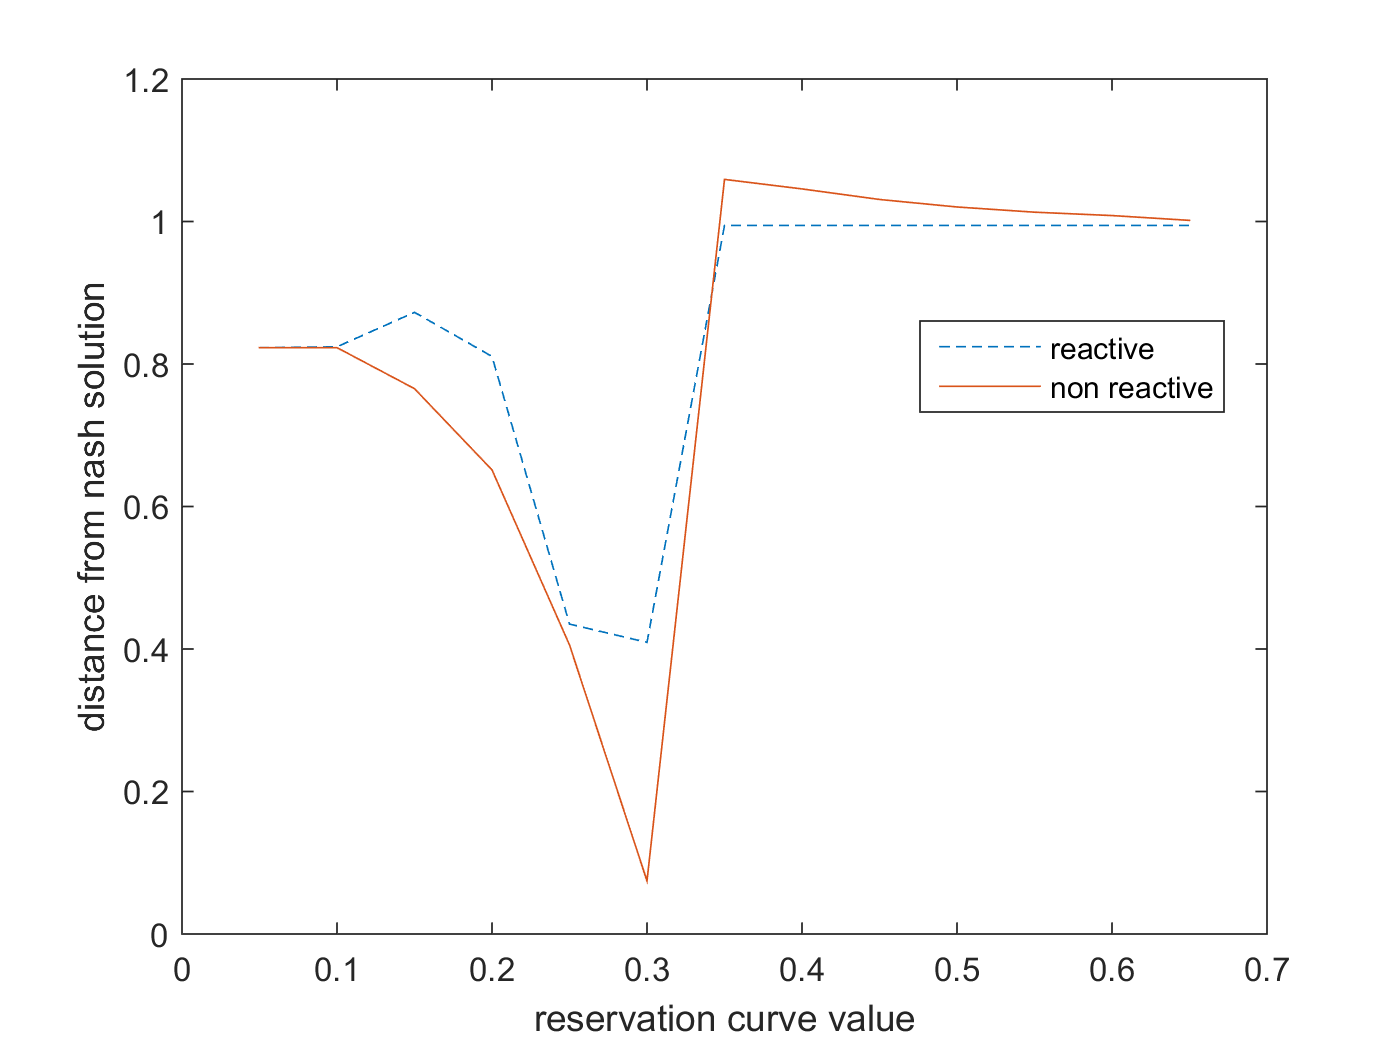
\includegraphics[width=0.9\linewidth]{img/reactivevsnonreactive}
	\caption{Distance from the Nash bargaining solution for the reactive and non-reactive concession strategies. }
	\label{fig:reactivevsnon-reactive}
\end{figure}

When looking at the distance and the amount of rounds necessary to find an solution (\Cref{tab:reactivevsnon-reactive}), we see that although our Nash limit lies at 0.3182, this solution is not found if the reactive concession strategy is used. 

\npdecimalsign{.}
\nprounddigits{4}
\begin{table}[h]
\begin{tabular}{|l|n{1}{4}|c|n{1}{4}|c|}
	\hline 
	&	\multicolumn{2}{|c|}{Reactive concession}&\multicolumn{2}{|c|}{Non-reactive concession}\\
	\cline{2-5}
{{reservation utility}}	& {{distance}} & {{\# of rounds}}  & {{distance}} & {{\# of rounds}} \\ 
	\hline 
0.05&	0&				26&		0.0295631273025621&		23\\
0.10&	0&				26&		0.0295631273025621&	 	23\\
0.15&	0&				38&		0.0295631273025621&	 	23\\
0.20&	0&				50&		0.0295631273025621&	 	23\\
0.25&	1.06932375691321&199&	0.0295631273025621&		23\\
0.30&	1.17512099855347&199&	0.0485167717872400&		66\\
0.35&	1.17163511966245&199&	0.127686769276389 &		199\\
0.40&	1.16753472222222&199&	0.279876154743691 &		199\\
0.45&	1.16753472222222&199&	0.425372845848635 &		199\\
0.50&	1.16753472222222&199&	0.555524071073009 &		199\\
0.55&	1.16753472222222&199&	0.673260175537175 &		199\\
0.60&	1.16753472222222&199&	0.780744817700835 &		199\\
0.65&	1.16753472222222&199&	0.874525088634732 &		199\\
%0.05&0					&0					&71	&71\\
%0.10&0					&0					&71	&71\\
%0.15&0					&0					&75	&71\\
%0.20&1.14485680268108	&0					&199	&71\\
%0.25&1.16166491047958	&0					&199	&71\\
%0.30&1.16559088622915	&0					&199	&71\\
%0.35&1.16828500771129	&0.127686769276389	&199	&199\\
%0.40&1.16753472222222	&0.279876154743691	&199	&199\\
%0.45&1.16753472222222	&0.425372845848635	&199	&199\\
%0.50&1.16753472222222	&0.555524071073009	&199	&199\\
%0.55&1.16753472222222	&0.673260175537175	&199	&199\\
%0.60 &1.16753472222222	&0.780744817700835	&199	&199\\
%0.65&1.16753472222222	&0.874525088634732	&199	&199\\
\hline
\end{tabular} 
\caption{The distance in the final proposal and number of rounds of a simulation.}
\label{tab:reactivevsnon-reactive}
\end{table}
\npnoround

It is very interesting to see that the non-reactive concession strategy halts after 23 rounds, which means that it is faster than the reactive concessions strategy. It also has some distance, which means that there is no real agreement, since the distance is larger than 0. However, when looking at the distance from the reactive concession, it is zero, which means that the average is exactly the same as the proposals. Interestingly when looking at the distance from the optimal solution, \Cref{fig:reactivevsnon-reactive}, it is very large. This unexpected result will be discussed later. 
\section{Reactive mixbed vs non-reactive }
Although the reactive concession strategy performed worse when compared to the non-reactive concession strategy, a comparison to is made when only the mixbed agent uses the reactive strategy. The mixbed agent is the most important agent since it ``produces'' the final demi water product.

In the comparison of the Nash Bargaining Solution, in \Cref{fig:reactivevsnon-reactivevsnon-reactivemxbrea} it is seen that the method initially performs better than the reactive strategy. 


\begin{figure}[h]
	\centering
	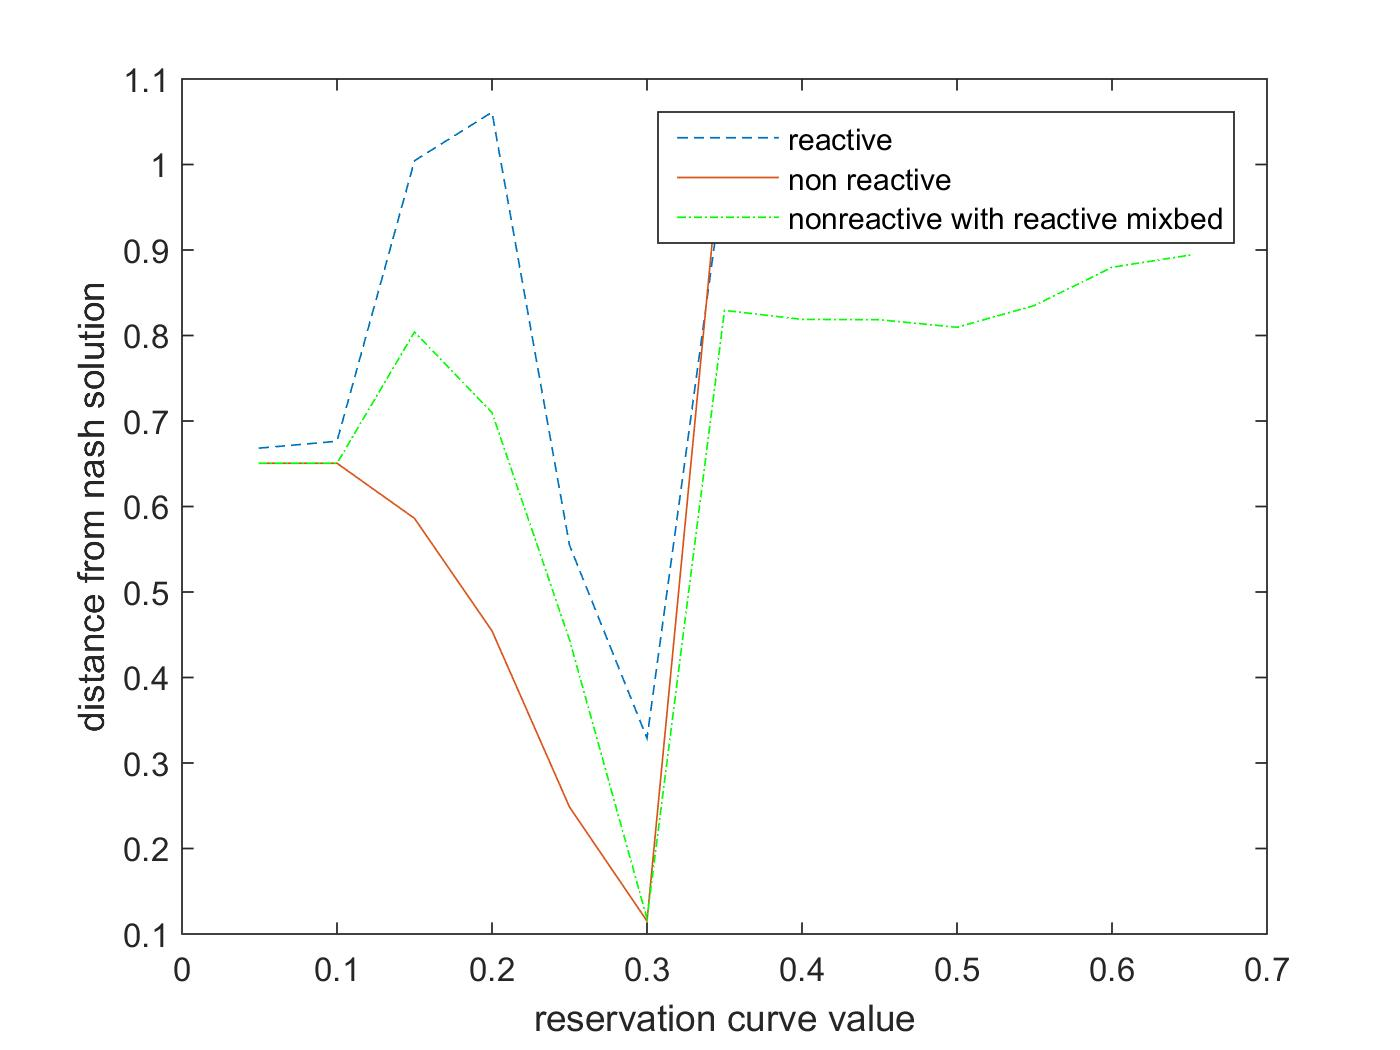
\includegraphics[width=0.9\linewidth]{img/reactivevsnonreactivevsmixbedrea}
	\caption{Comparison of the reactive and non-reactive vs only reactive mixb}
	\label{fig:reactivevsnon-reactivevsnon-reactivemxbrea}
\end{figure}

The table of the distance and number of rounds is very repetitive. Exactly the same, although the end solution, which is the average of all offers, is close to the Nash solution. It does not find the solution within the 200 rounds however.

\npdecimalsign{.}
\nprounddigits{4}
\begin{table}[h]
	\centering
\begin{tabular}{|c|n{1}{4}|c|}
	\hline 
	reservation utility	& {distance} & \# of rounds \\ 
	\hline 
	
	0.05&1.18691980311553 & 199\\
	0.10&1.18691980311553 & 199\\
	0.15&1.18691980311553 & 199\\
	0.20&1.18691980311553 & 199\\
	0.25&1.18691980311553 & 199\\
	0.30&1.18691980311553 & 199\\
	0.35&1.18691980311553 & 199\\
	0.40&1.18691980311553 & 199\\
	0.45&1.18691980311553 & 199\\
	0.50&1.18691980311553 & 199\\
	0.55&1.18691980311553 & 199\\
	0.60&1.18691980311553 & 199\\
	0.65&1.18691980311553 & 199\\
	\hline
\end{tabular} 
\caption{The distance in the final proposal and number of rounds of a simulation. This is where only the mixbed makes reactive concessions, and the other agents make non-reactive concessions.}
\label{tab:reactivevsnon-reactivevsmixbedrea}
\end{table}
\npnoround

\section{Changing the $l$ value for the mixbed}
In the design it was stated that the water ratio to the base and acid could change for the mixbed. Here an example is given where the mixbed water to base and acid ratio is 2:1:1 and 10:1:1. Here a new Nash solution has to be calculated, since the utility functions have changed. So in the graph comparison, the mixbed water with the updated ratio, is checked against the reactive and non-reactive concession strategies.

\subsection{Mixbed 2 water}
When looking at the first ration of 2:1:1, we get very similar result as that of the comparison. The minimum $rui$ lies way lower however, and has an maximum of $\forall i, ru_i = 0.301$. The Nash solution lies at acid = 0.600, base = 0.600, water = 0.800.
It is interesting to note that the new original end proposal is a lot nearer to the Nash solution than the base line situation when the reservation utility is low as can be seen in \Cref{fig:reactivevsnon-reactivemixbed2}. Again the non-reactive concession strategy comes closer to the Nash solution ultimately, however initially the reactive concession strategy is better. 
\begin{figure}[h]
	\centering
	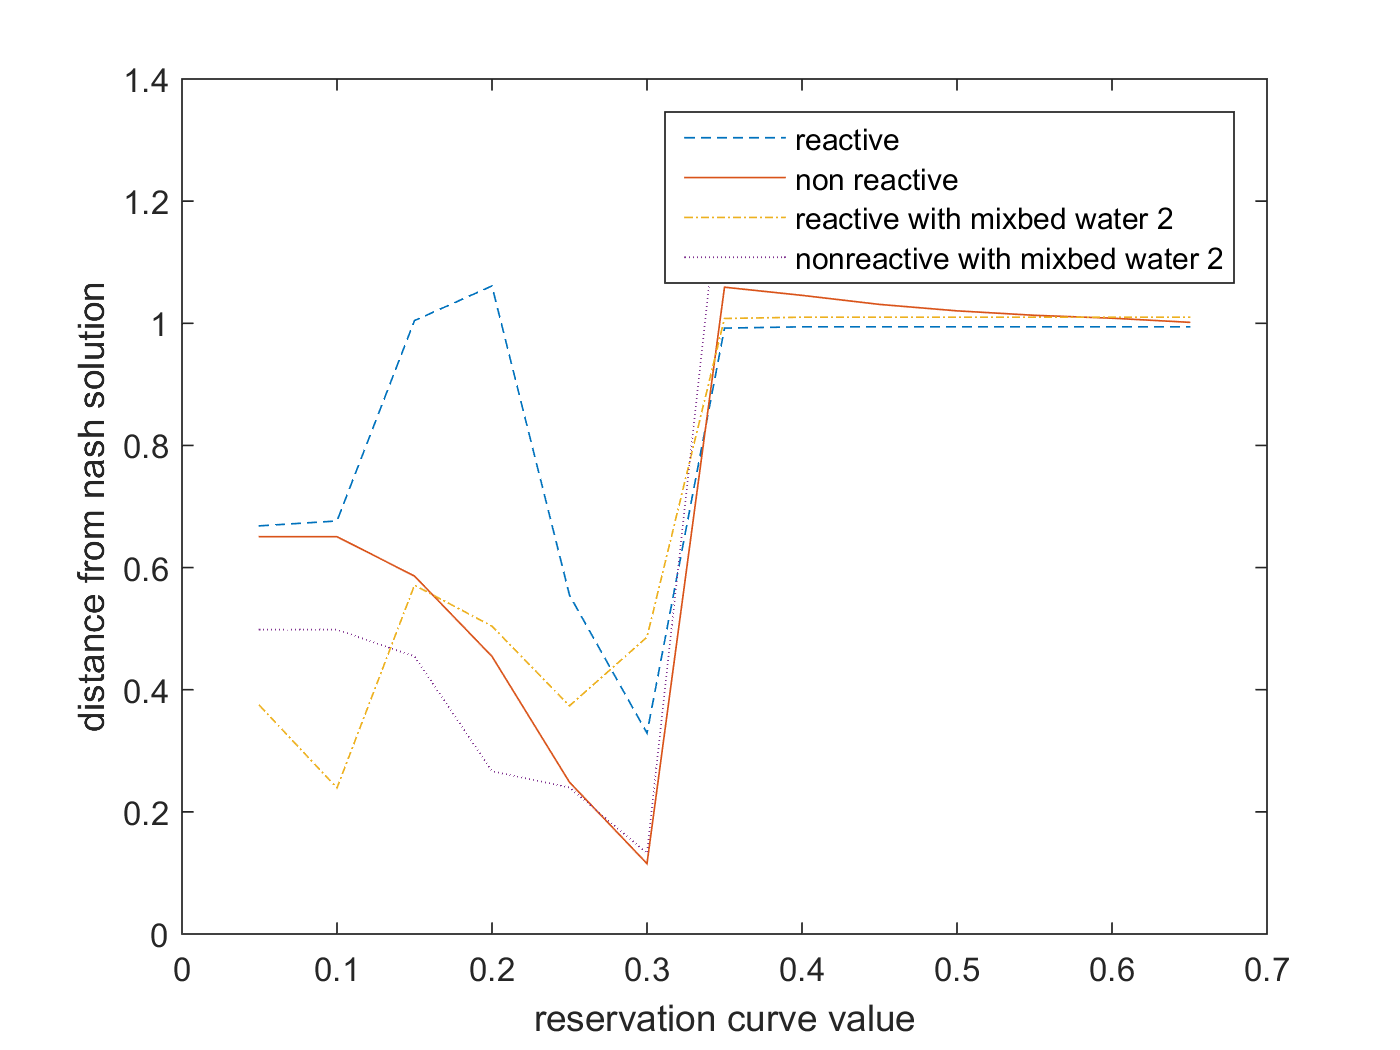
\includegraphics[width=0.7\linewidth]{img/reactivevsnonreactivemixbed2.png}
	\caption{Comparison of the reactive and non-reactive strategy for a 2 water value mixbed.}
	\label{fig:reactivevsnon-reactivemixbed2}
\end{figure}


\npdecimalsign{.}
\nprounddigits{4}
\begin{table}

\begin{tabular}{|l|n{1}{4}|c|n{1}{4}|c|}
	\hline 
		&	\multicolumn{2}{|c|}{Reactive concession}&\multicolumn{2}{|c|}{Non-reactive concession}\\
	\cline{2-5}
	{{reservation utility}}	& {{distance}} & {{\# of rounds}}  & {{distance}} & {{\# of rounds}} \\ 
	\hline 
0.05 & 0                 & 26  & 0                  & 26  \\
0.10 & 0                 & 30  & 0                  & 26  \\
0.15 & 0                 & 43  & 0                  & 26  \\
0.20 & 0.950693168831420 & 199 & 0                  & 26  \\
0.25 & 1.11331450231946  & 199 & 0                  & 26  \\
0.30 & 1.24151874372075  & 199 & 0.0472373495100384 & 71  \\
0.35 & 1.24001645374814  & 199 & 0.282988815136597  & 199 \\
0.40 & 1.23596954345703  & 199 & 0.452220659395809  & 199 \\
0.45 & 1.23596954345703  & 199 & 0.677438159537665  & 199 \\
0.50 & 1.23596954345703  & 199 & 0.779689267474365  & 199 \\
0.55 & 1.23596954345703  & 199 & 0.862468304051885  & 199 \\
0.60 & 1.23596954345703  & 199 & 0.926781060892920  & 199 \\
0.65 & 1.23596954345703  & 199 & 0.985943062172507  & 199\\
\hline
\end{tabular}
\label{tab:mixbed2}
\caption{Here mixbed is water 2. }
\end{table}
\npnoround


\subsection{Mixbed 10 water}
When using an ratio of 10:1:1 we have an max $ru_i = 0.274$. The Nash solution lies at acid = 0.647, base = 0.647, water =0.941. The large increase to the water demand makes this an interesting solution. It is very interesting to note that although the reservation minimum lies at $0.274$, the algorightm still finds an solution very close to the Nash optimum when the reservation utility is 0.3. 
%\section{All}

\begin{figure}[h]
	\centering
	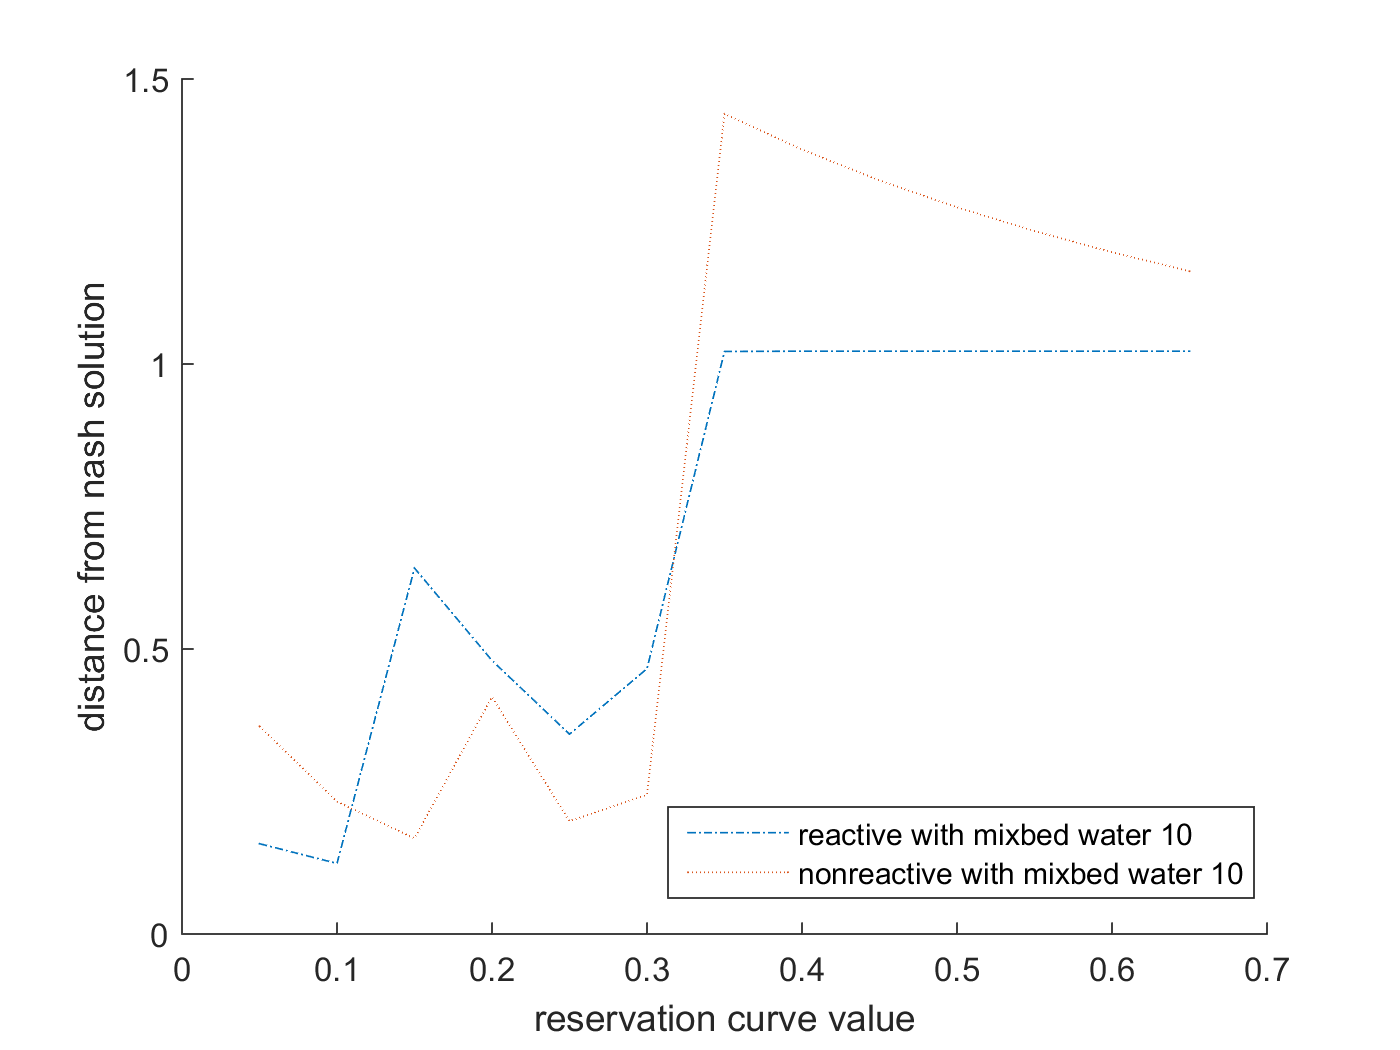
\includegraphics[width=0.7\linewidth]{img/reactivevsnonreactive_mixbed10}
	\caption{Comparison of the reactive and non-reactive strategy for a 10 water value mixbed.}
	\label{fig:reactivevsnonreactivemixbed10}
\end{figure}

\npdecimalsign{.}
\nprounddigits{4}
\begin{table}[h]
	\centering
\begin{tabular}{|l|n{1}{4}|c|n{1}{4}|c|}
	\hline 
	&	\multicolumn{2}{|c|}{Reactive concession}&\multicolumn{2}{|c|}{Non-reactive concession}\\
\cline{2-5}
{{reservation utility}}	& {{distance}} & {{\# of rounds}}  & {{distance}} & {{\# of rounds}} \\ 
\hline 
0.05 & 0                & 34  & 0                  & 26  \\
0.10  & 0                & 38  & 0                  & 30  \\
0.15  & 0                & 59  & 0                  & 30  \\
0.20  & 1.01017004837544 & 199 & 0.0375849182069237 & 47  \\
0.25  & 1.18451892325133 & 199 & 0.0403767460130609 & 59  \\
0.30  & 1.28304255654208 & 199 & 0.196731504342998  & 199 \\
0.35  & 1.30000 & 199 & 0.516805014278959  & 199 \\
0.40  & 1.30000 & 199 & 0.620662764097981  & 199 \\
0.45  & 1.30000 & 199 & 0.712271791830695  & 199 \\
0.50  & 1.30000 & 199 & 0.794218859564544  & 199 \\
0.55  & 1.30000 & 199 & 0.868348999412338  & 199 \\
0.60  & 1.30000 & 199 & 0.936024514848705  & 199 \\
0.65  & 1.30000 & 199 & 0.998279954150336  & 199\\
\hline
\end{tabular}
\label{tab:mixbed10}
\caption{Here mixbed is water 10. }
\end{table}
\npnoround
%\begin{figure}
%	\centering
%	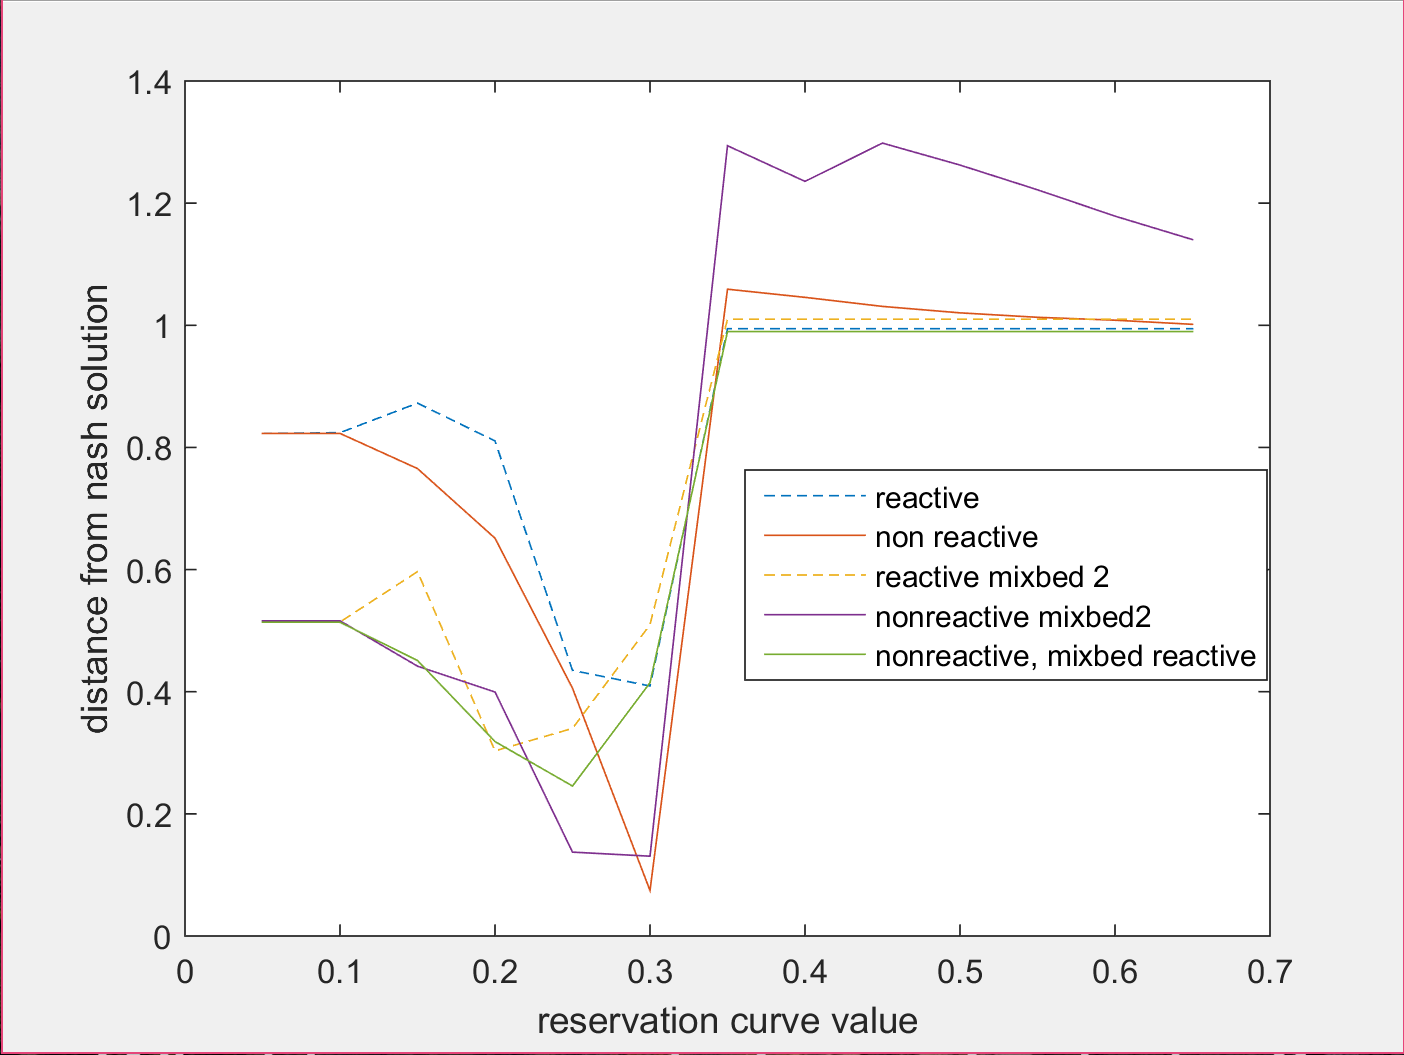
\includegraphics[width=0.7\linewidth]{img/all_dist_from_nash_solutions}
%	\caption{All plots fromthe nash solutions.}
%	\label{fig:alldistfromnashsolutions}
%\end{figure}

\clearpage
\section{Discussion}
\subsection{reactive vs non-reactive}
A possible solution is that the answer can not be found as is stated by \citet{zheng2015automated} as Lemma 2. ``If Agent i deliberately stops conceding before reaching the agent's own reservation utility from time period t onward. and all other agents use the reactive concession strategy the negotiation will stall; i.e. other agents will reactively stop conceding and there will be no agreement. if $\Delta_j < s_j(t)-u_j(x^*_{ru_i}) \text{ and } u_j(x^*_{s_i(t)})<ru_j$''.

This is although there is a nonempty zone of agreement it does not find it. This can be clearly seen when we analyze the situation for the reservation curve at 0.2.

\subsubsection{Situation at the 0.2 ru}
So as shown in the results. there is a unexpected distance from the Nash solution in the situation of the 0.2 reservation curve. This can mostly be attributed to the stalling of the agents while trying to find a solution.

Looking at the proposals made. it is clearly seen that in the reactive process. the Neut and Mixbed do not react to the proposals of the Anion and Cation. After multiple proposals they finally adjust 

\begin{figure}[h]
	\centering
	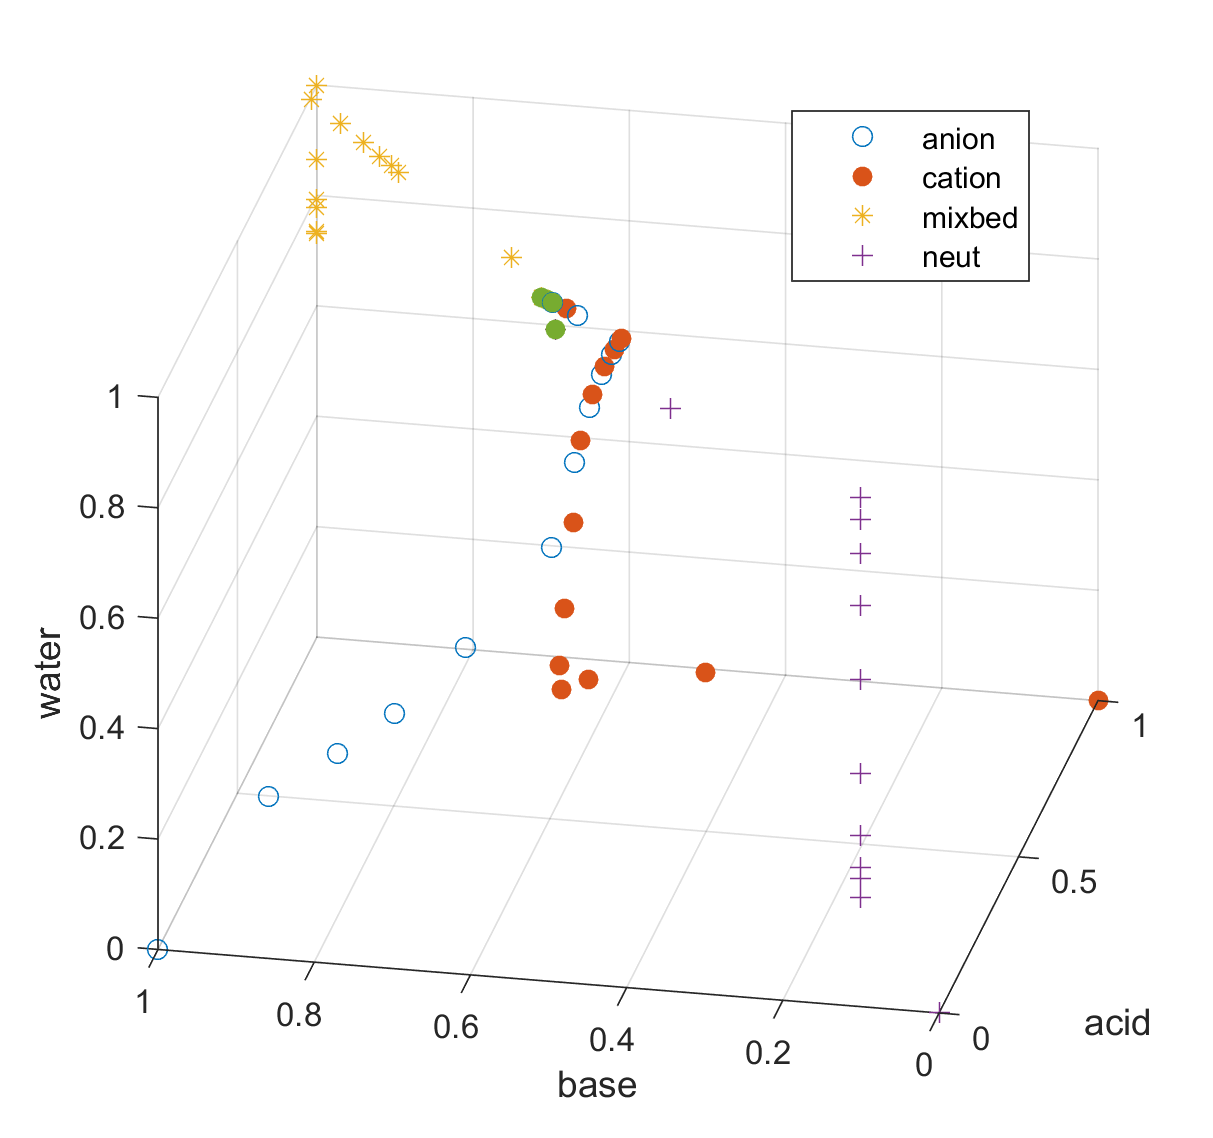
\includegraphics[width=0.7\linewidth]{img/reactive_4_plot}
	\caption{The proposals made by the 4 agents. We see that the mixbed and neut ``stall'' in de finding of the solution.}
	\label{fig:reactive4plot}
\end{figure}

\begin{figure}[h]
	\centering
	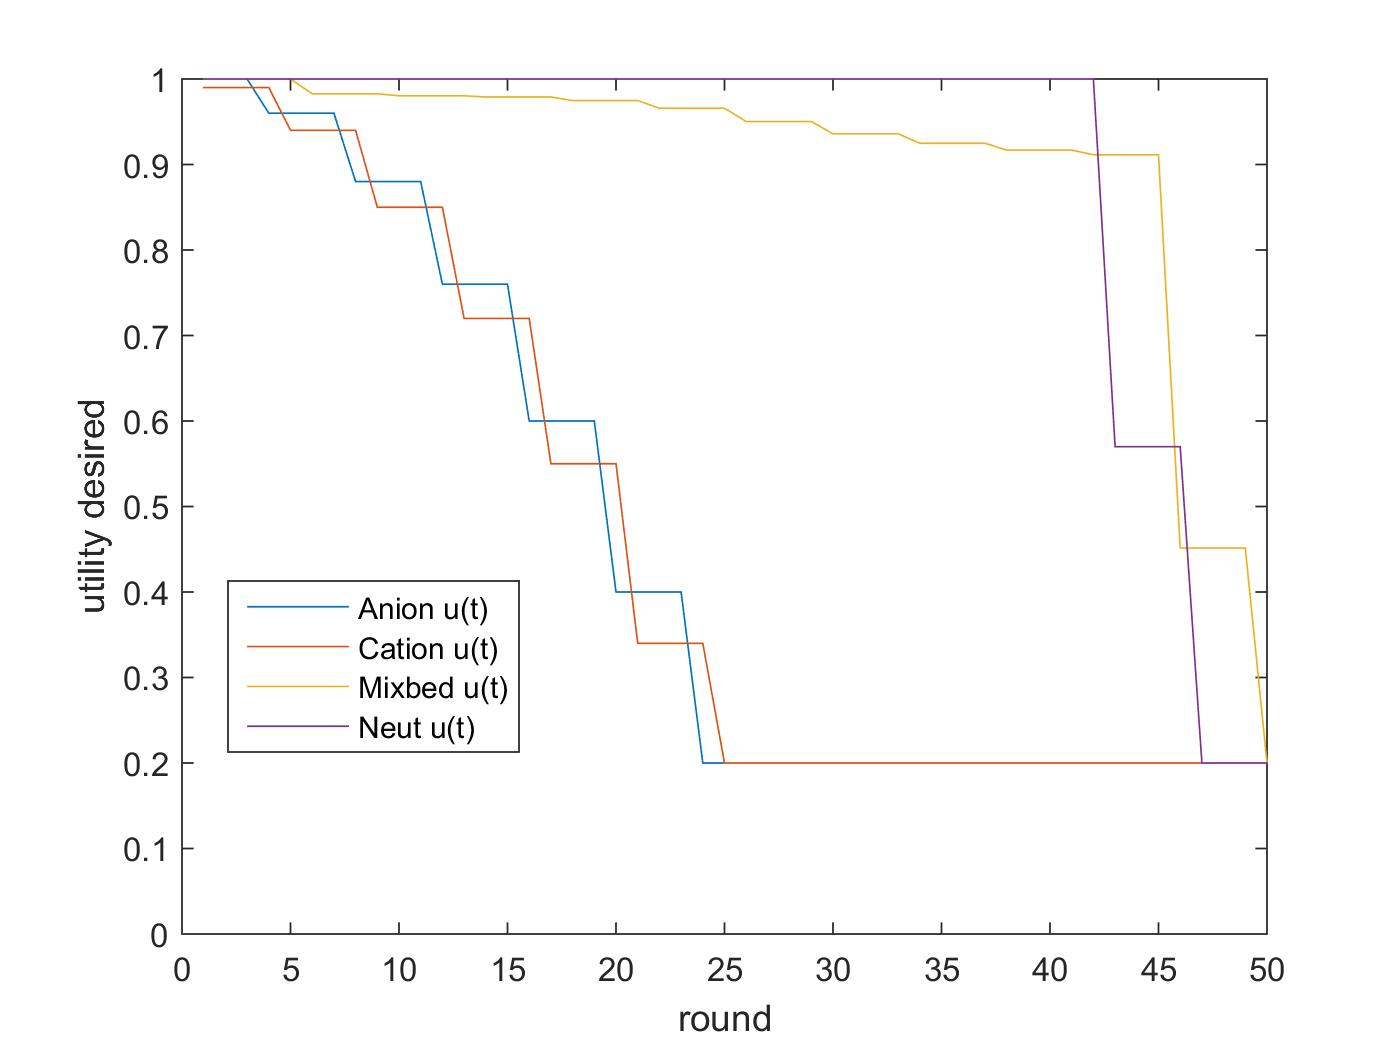
\includegraphics[width=0.7\linewidth]{img/desiredutility_reactive_4}
	\caption{The desired utility for the agents. The stall can be clearly seen for the mixbed and neut agent. Only towards the end do they start conceding.}
	\label{fig:desiredutilityreactive4}
\end{figure}

\paragraph{The solution space}

\section{Solution space}
Below the solution space for the agents is shown, when $ru_i = 0.2$ for all agents. Each agent has 2 or three subjects. 
\begin{figure}[h]
	\centering
	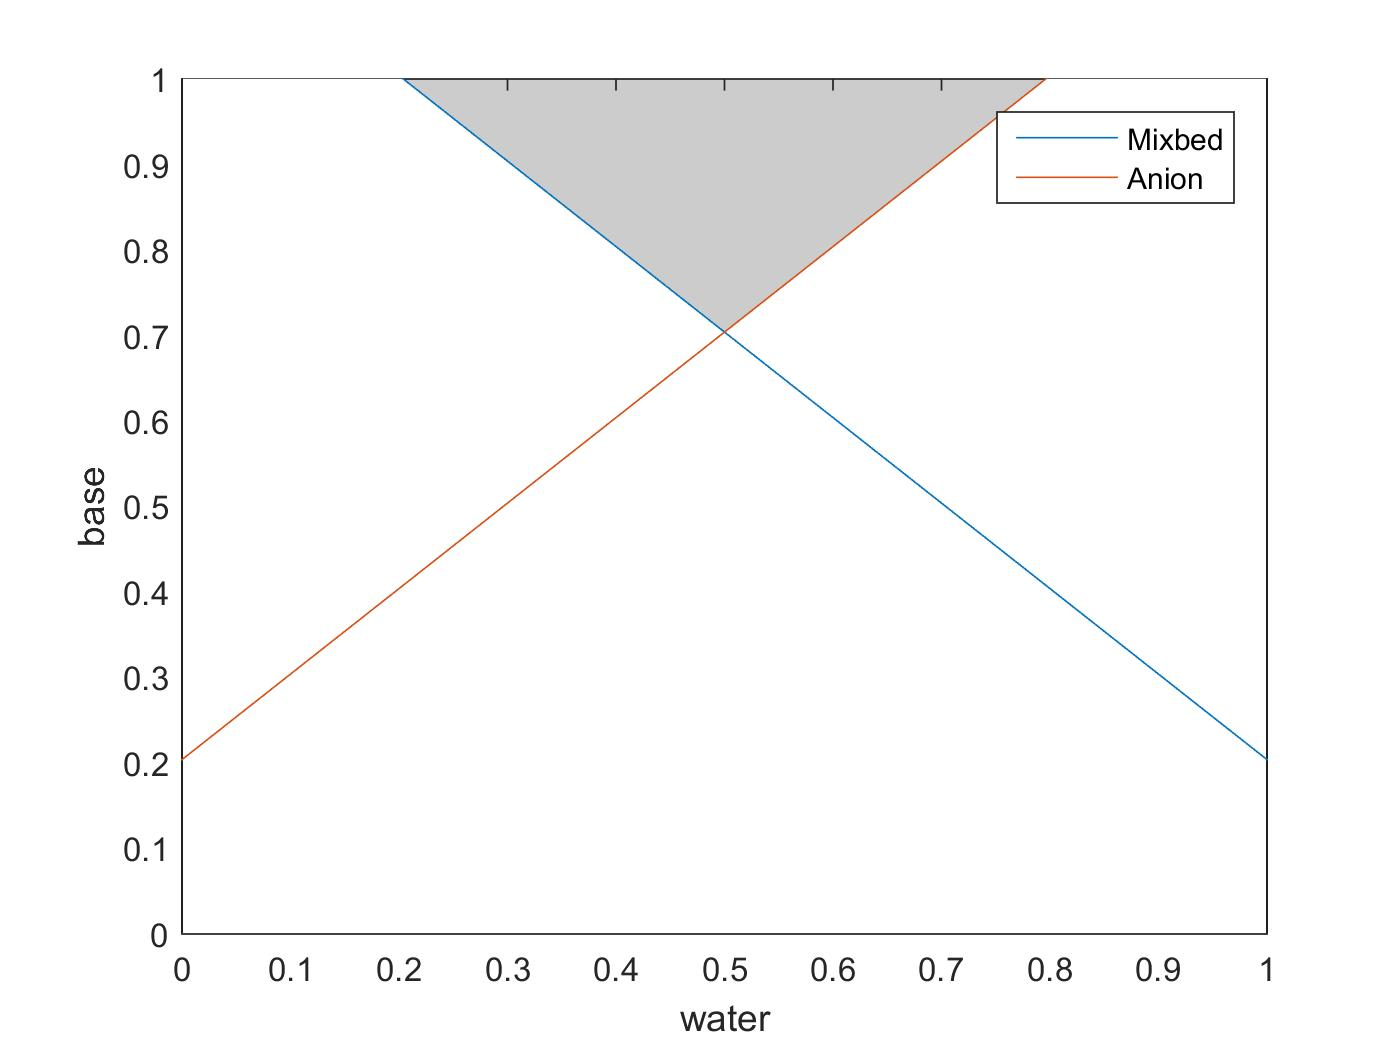
\includegraphics[width=0.7\linewidth]{img/reservationcurve_water_base}
	\caption{The solution space for the combination of base and water, which are negotiated over by the anion and the mixbed agent.}
	\label{fig:reservationcurvewaterbase}
\end{figure}

\begin{figure}[h]
	\centering
	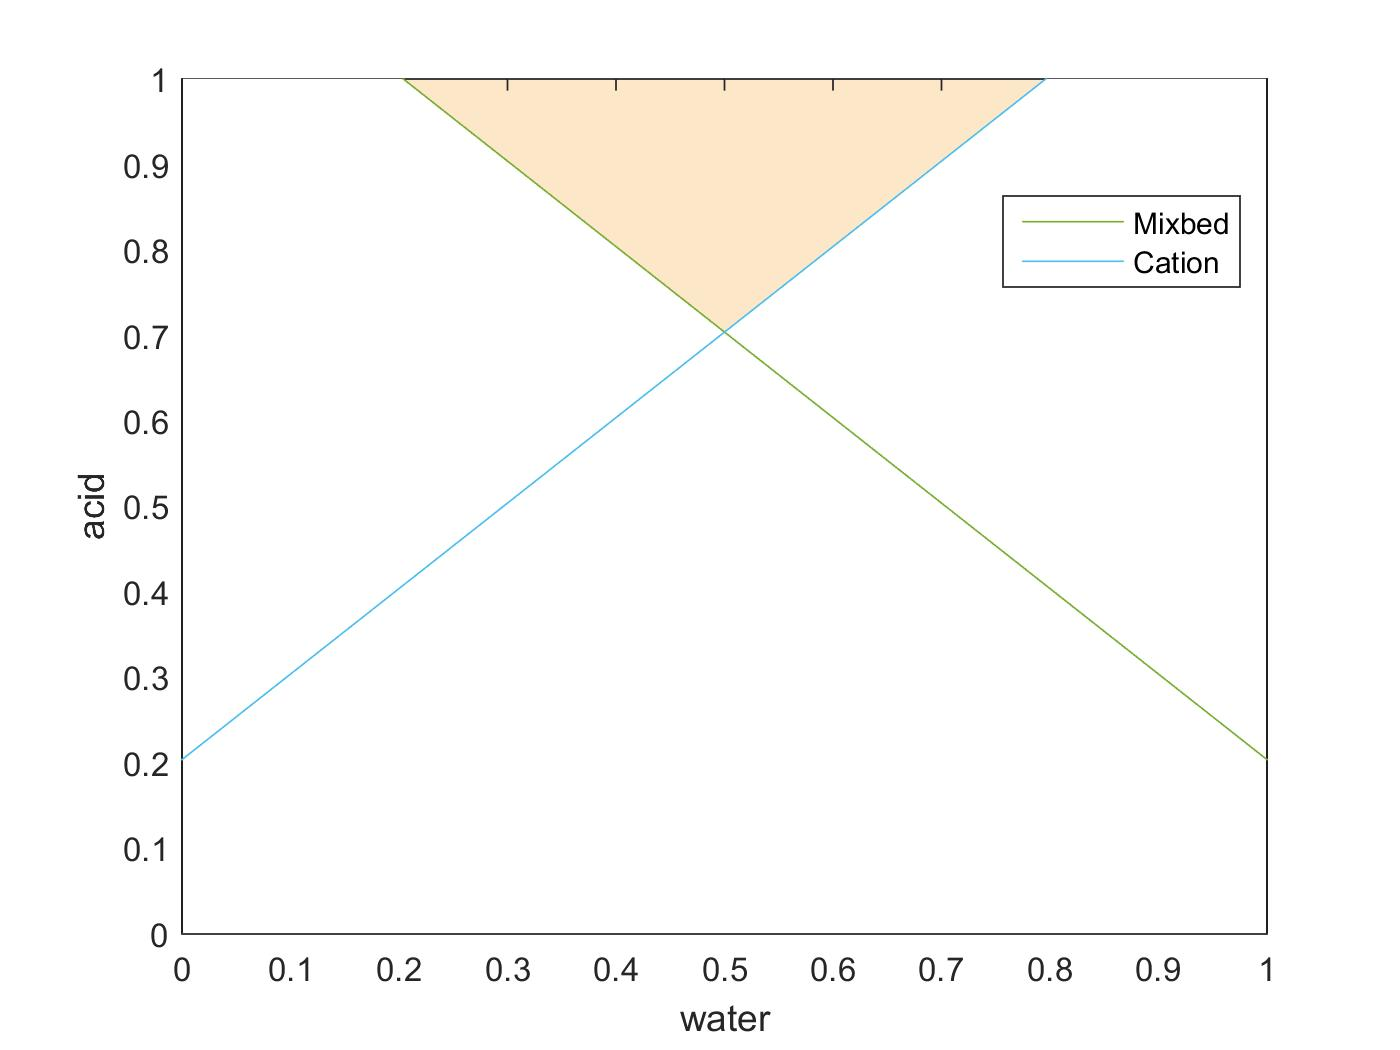
\includegraphics[width=0.7\linewidth]{img/reservationcurve_water_acid}
	\caption{The solution space for the combination of acid and water}
	\label{fig:reservationcurvewateracid}
\end{figure}
\begin{figure}[h]
	\centering
	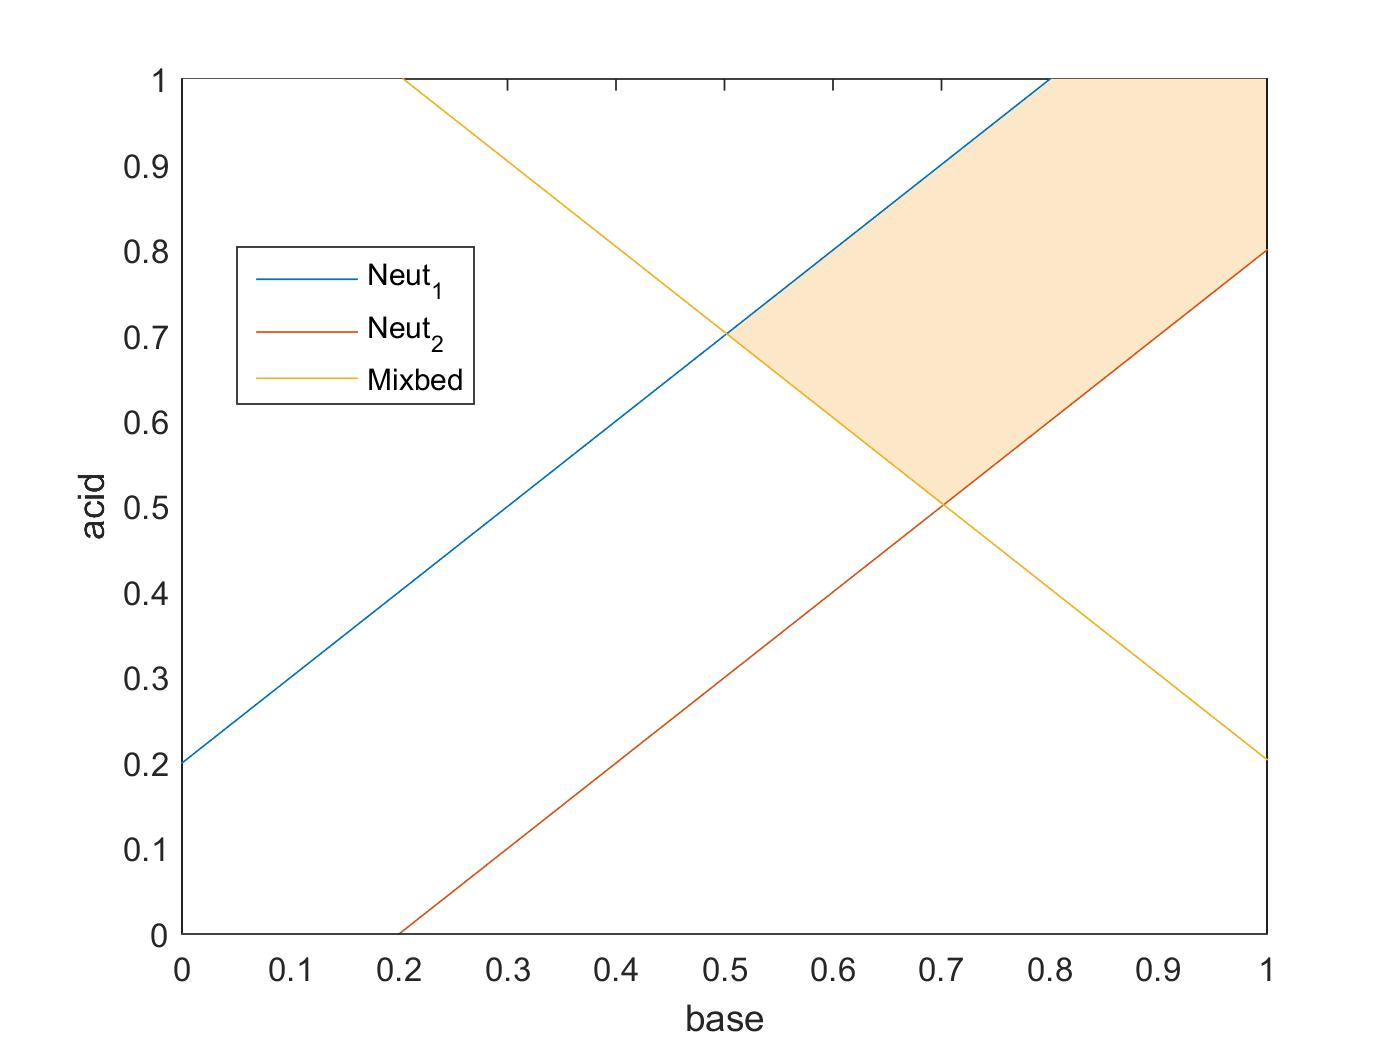
\includegraphics[width=0.7\linewidth]{img/reservationcurve_base_acid}
	\caption{The solution space for the combination of acid and base}
	\label{fig:reservationcurvebaseacid}
\end{figure}


\subsection{reactive mixbed vs non-reactive}
Nash solution lies in 0 water with 1 base and 1 acid. This is close to the start of mixbed in 1.1.1

This is however the result of the stalling of the mixbed. and not the result of the solution being found. This is obvious when looking at the table. Although the reservation curve changes in the offers. the mixbed does not move. This can also been seen in the proposal figure

\todo[Todo Hier proposal figure toevoegen]{Hier proposal figure toevoegen!!}


